\documentclass[11pt,a4paper]{article}
\usepackage[T1]{fontenc}
\usepackage{isabelle,isabellesym}

% this should be the last package used
\usepackage{pdfsetup}
\usepackage{graphicx}
% urls in roman style, theory text in math-similar italics
\urlstyle{rm}
\isabellestyle{it}
\renewcommand{\isasymacute}{\isatext{\'\relax\hspace{-0.20em}}}
\DeclareRobustCommand{\isactrlesup}{\egroup\egroup\endmath\egroup\relax\hspace{-0.15em}}

\begin{document}

\title{BDD-Normalisation}
\author{Veronika Ortner and Norbert Schirmer}
\begin{abstract}
We present the verification of the normalisation of a binary decision
diagram (BDD). The normalisation follows the original algorithm
presented by Bryant in 1986 and transforms an ordered BDD in a
reduced, ordered and shared BDD. The verification is based on Hoare
logics.
\end{abstract}
\maketitle

\tableofcontents
\begin{center}
  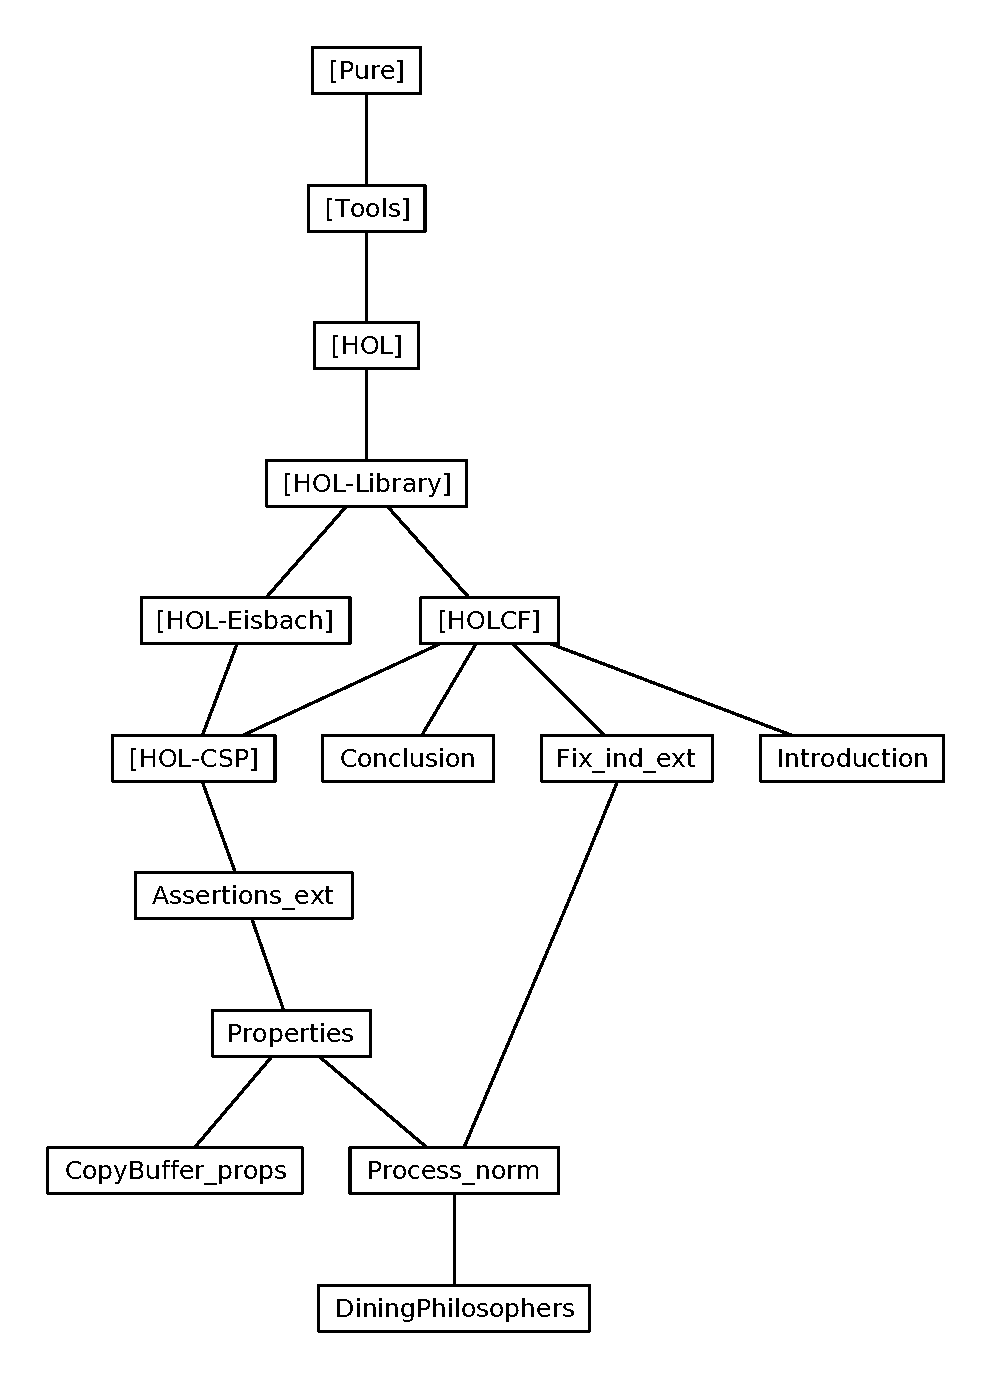
\includegraphics[width=\textwidth=\textheight,keepaspectratio]{session_graph}
\end{center}
\parindent 0pt\parskip 0.5ex

\section{Introduction}

In \cite{Ortner-Schirmer-TPHOL05} we describe the partial correctness proofs for
BDD normalisation. We extend this work to total correctness in these theories.


% generated text of all theories
\input{session}

% optional bibliography
\bibliographystyle{abbrv}
\bibliography{root}

\end{document}

%%% Local Variables:
%%% mode: latex
%%% TeX-master: t
%%% End:
